\documentclass{sigkddExp}
\usepackage{tabularx}
    \newcolumntype{L}{>{\raggedright\arraybackslash}X}

\begin{document}

\title{Neural networks for card transactions analysis}

\numberofauthors{1}
\author{
\alignauthor Anonymous authors
Paper under double-blind review
}

\date{30 July 1999}
\maketitle
\begin{abstract}
In this paper we'd like to describe our successful attempt to use neural networks in conservative credit scoring domain.
The goal is to predict should we accept an application for a credit using the clients card transaction history.
\end{abstract}

\section{Introduction}
Traditionally, very simple models like logistic regression are used for the task of credit scoring. They are easily interpretable, computationally effective and have modest requirements to the dataset volume.

Unfortunately such models do not easily apply to some types of valuable data. History of card transactions is a good example. Nearly half of the clients coming to take a credit already have some type of card account in the bank. And the transactions of that client contain information that can be used to predict customer credibility in addition to commonly used data such as credit history data and questionary data. One way to integrate such data into existing models would be by creating a number of aggregate variables (mean number of transactions per day, mean transaction amounts, mean balance etc.) In this paper we use a neural network to process transactional data without creating intermediate aggregates.

\section{Related work}

While neural networks operating on raw transactional level data are used for the task of detection of fraudulent transactions for more than a decade \cite{fraud_lstm} we have not been able to find any usage of such data for the credit scoring task. Such data is incorporated either through some intermediate aggregation, use only the connectivity graph\cite{RePEc} or are recently used in a similar task of prediciting credit rations on p2p lending platforms.

To our knowledge this is the first time raw transaction-level bank data is used for the task of credit scoring. 

\section{Our approach}
\subsection{Data preparation}


Each client has multiple time-stamped transactions and each transaction has several attributes, both categorical and numeric. See an example in table \ref{tab1}. Hence, our data looks like multivariate time-series, which is not the best representation for classical ML algorithms like logistic regression.

\begin{table}
\caption{Data structure for a single client}
\begin{tabular}{ | l |  l l l | }
\hline
\textbf{Amount} & 230 & 500 & 540 \\
\textbf{Currency} & EUR & RUR & RUR \\
\textbf{Country} & France & Russia & Russia \\
\textbf{Time} & 16:40 & 20:15 & 09:30 \\
\textbf{Date} & Jun 21 & Jun 21 & Jun 22 \\
 & 5813 & 4111 & 5722 \\
\textbf{MCC} & (Drinking & (Transport) & (Household \\
 & Places) &  & Appliance) \\
\textbf{Card type} & Visa Classic & Visa Classic & Visa Gold \\
\textbf{Issuing} & 90/10735 & 90/01735 & 90/01779 \\
\textbf{Branch} &&& \\
\hline
\end{tabular}
\label{tab1}
\end{table}

Each categorical variable in each transaction is encoded to a low-dimensional vector via embedding layers. We have treated the timestamp as a collection of categorical variables each representing a date part (hour, weekday, month). Each transaction is represented with a concatenation of scalar variables and embeddings of categorical variables. Each client is represented by a sequence of transactions.
The avaivable transaction data falls into 

\scategories - transaction-level (timestamp, country, amount, MCC) and card-level (issuing branch, card type), card-level data is duplicated verbatim for each transaction corresponding to the said carubsection{Experiment data}
Our tratwo ining dad.. taset represented XX M  users with XX M total transactions. As a target variable we used the event of default for consumer loan during a year after its disbursement. 
We have used data for period XX - XX for training  (XX applications, XX defaults) and period XX -XX for out-of-time validation (XX applications, XX defaults ) Due to a large disparity between number of positive and negative cases we settled on the following sampling strategy: before each experiment select all positive cases and 10 times as much randomly selected negative cases, on each training epoch we use all positive cases and a same number of negative cases, selected from the negative cases pool.  

\subsection{Architecture overview}
The general idea was to produce low-dimensional representation of the time-series and then pass it to a classifier. Then it would be possible to perform end-to-end training of the whole network including embeddings, encoder and classifier.

\subsubsection{Embeddings}

Categorical variables are embedded into a latent space before being passed to the encoder. The embedding layers are randomly ititialized and trained simultaneously with the encoder.
The dimensionality of such embedding layer is an important hyperparameter as the number of trainable weights in embedding layer is significantly bigger than the number of weights in the encoder.  

Graph: Ox-epoch, Oy-Train/Validation Gini , Series: (small, medium, big)

\subsubsection{Encoder}

We tried two approaches. The first was a bag-of-transactions model where each separate attribute of the transaction vector was averaged across all transactions of a person to form the client representation. The second approach was to pass transaction vectors to RNN one by one and use RNN as an encoder. The hidden vector from the last last time step was used as the representation. This approach as typically used for text analysis “Sequence to Sequence Learning with Neural Networks”\cite{NIPS2014_5346}.

\begin{table}
\caption{Encoder architecture comparison}
\begin{tabular}{ | l | c |  }
\hline
& \textbf{validation Gini} \\
\hline
\textbf{GRU 1-layer} & 0,62  \\
\textbf{GRU 2-layer} & 0,67  \\
\textbf{LSTM 1-layer} & 0,67  \\
\textbf{LSTM 2-layer} & 0,67  \\
\textbf{GRU 1-layer Bidirectional} & 0,67  \\
\hline
\end{tabular}
\label{tab3}
\end{table}

\subsubsection{Classifier}

We tried several classifiers based on multi-layer perceptrons with different activation functions, but were not able to archive better results than with a simple linear classifier.

\subsection{Transaction count}

\begin{figure}
  \caption{Around 100 transactions is enough for confident classification}
  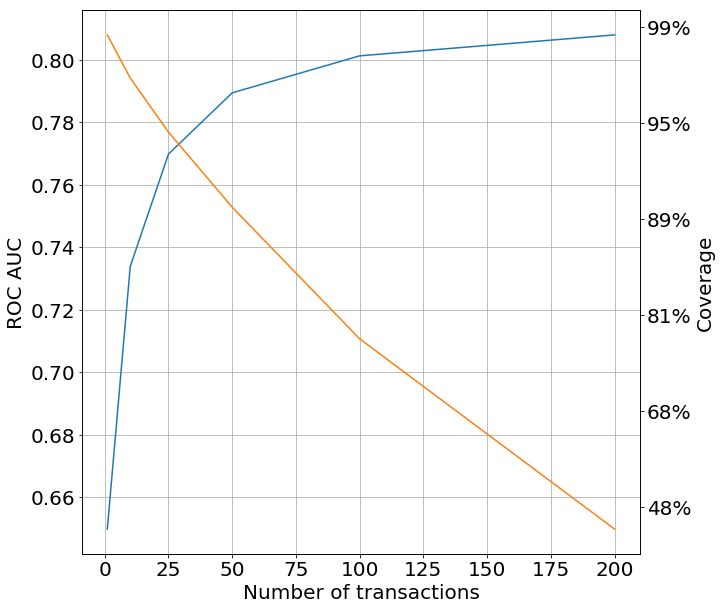
\includegraphics[width=0.46\textwidth]{information-vs-accuracy.png}
  \label{fig2}
\end{figure}

Also we can see on figure\ref{fig2} that one hundred transactions is enough to confidently estimate the default probability of a client. Half of the clients with plastic card have more than one hundred transactions. All models in this paper where trained on last 800 transactions, padding by zero when the actual transaction count for a client was lower.

\subsection{Loss function}

Our quality metric was Gini which is the scaled variant of ROC AUC ($G = 2A_{ROC} - 1$). Gini is the most popular metric for the credit scoring task.

Several loss functions can be used as a proxy for the task of maximising Gini. The classic binary cross-entry loss: $L_{CE}(p, y) = - \sum_i y_ilog(p_i)$ is the default choice.
The other possible approach is to use ranking loss: $ L_R(p_1, p_2, y) = \max(0, -y * (p_1 - p_2) + margin $ which directly optimizes Gini.

There is also an option to use modified version of binary cross-entropy loss proposed by Lin et al.\cite{DBLP:journals/corr/abs-1708-02002} and known as focal loss: $L_F(p, y) = -\sum_i (1 - p_i)^\gamma y_i log(p_i)$. Focal loss reduces penalty for easily classified samples i. e. samples for which the model prediction is very close to one. This is especially actual for poorly balanced datasets which is exactly our case. But preliminary tests of focal loss showed no improvement against BCE loss.

For production version we used margin ranking loss with margin 0.01 which showed best results on the test data. 

\begin{table}
\caption{Loss comparison}
\begin{tabular}{ | l | c |  }
\hline
& \textbf{validation Gini} \\
\hline
\textbf{BCE Loss} & 0,62  \\
\textbf{Hinge loss 0.5} & 0,67  \\
\textbf{Hinge loss 0.1} & 0,67  \\
\textbf{Hinge loss 0.01} & 0,67  \\
\textbf{Hinge loss 0.01 + BCE Loss} & 0,67  \\
\hline
\end{tabular}
\label{tab4}
\end{table}

\subsection{Learning rate}

Learning rate is one of the most sensitive hyper-parameters which can dramatically change the performance of the model. We tried several learning rates and several learning rate reduction regimes. We found that the most effective strategy was using an aggressive learning rate reduction with gamma=0.5.
For all experimens we used a batch size of 32 for training and batch size of 768 for validation.

While there are several techniques to tune learning rate the interesting option is to use cyclical learning rates like proposed by Leslie N. Smith.\cite{DBLP:journals/corr/Smith15a}

Graph: Ox-epoch, Oy-Train/Validation Gini , Series: (lr=0.0001 const, lr decreasing g=0.8, g=0.5, cyclical g =0.5) 


\subsection{Ensembling}

Ensembling is a way to increase both quality of the model and its stability a the expense of time and computational power. We decided to use mean predictions of the ensemble of separately trained models. In our case we have abundance of the positive class samples and can use different subsamples of the negative class samples for each model. This approach brings significant performance and stability boost.

Another interesting approach is to use snapshots of the same model in the final ensemble as proposed by Huang et al.\cite{DBLP:journals/corr/HuangLPLHW17} It can significantly reduce training time since only one model should be trained. The training time was not a big deal in our case and the quality was worse than the the quality for ensemble for different models.

Yet another interesting possibility is to use stochastic weight averaging proposed by Izmailov et al.\cite{DBLP:journals/corr/LoshchilovH16a} This approach can significantly reduce inference time since only one model with averaged weights is used instead of the whole ensemble. But in our case ensemble of models trained on slightly different subsets of data was best in terms of quality.

Box-plot: Series = {Single, Ens-3, Ens-6  diff loss? } Cols = {val Gini + STD}
best hyperparams


\subsection{Regularization methods}

Due to the low number of positive classes all models exhibit a propensity for ovefitting. We tried different regularisation methods:

1. Transaction dropout - randomly removing a share of client transactions

2. Transaction shuffle - randomly permute the order of client transactions

3. Transaction concatenation - create synthetic training examples by concatenation of 
transaction histories for two clients from the same class

3. Embedding dropout - randomly zero some components after ambedding layer

4. Encoder dropout - randomly zero some components after encoder




Graph: Ox-epoch, Oy-Train/Validation Gini , Series: (baseline, trx do, emb do, emb shuffle,) 


\subsection{Variable importance}


Graph of variable importance


\section{Comparison with classical methods...}

Logreg(note st the tsble that the data is not directly comparable)

\subsection{GBM based approach}

To compare our model with other approaches to classification we have also implemented completely different model. We used gradient boosting machine (Friedman\cite{friedman2001greedy}) as the classifier which gets large vector of hand-crafted aggregate features as an input. An example of aggregate feature would be the mean spends in some category of merchants (e. g. hotels).
We used LightGBM\cite{Ke2017LightGBMAH} implementation of GBM algorithm and created nearly 7000 aggregate features per sample.

\begin{table}
\caption{Experiment comparison}
\begin{tabular}{ | l | c | c | }
\hline
& \textbf{Gini} & \textbf{N Features} \\
\hline
\textbf{LGBM on aggregate features} & 0,62 & $\sim7000$ \\
\textbf{RNN on detailed data} & 0,67 & 16 \\
\hline
\end{tabular}
\label{tab2}
\end{table}


The comparison of validation results can be seen in \ref{tab2}. Training and validation sets were the same for each model.  As you can see RNN can significantly outperform classical ML approaches with hand-crafted features given enough data.

\begin{figure}
  \caption{RNN has steeper learning curve than LGBM.}
  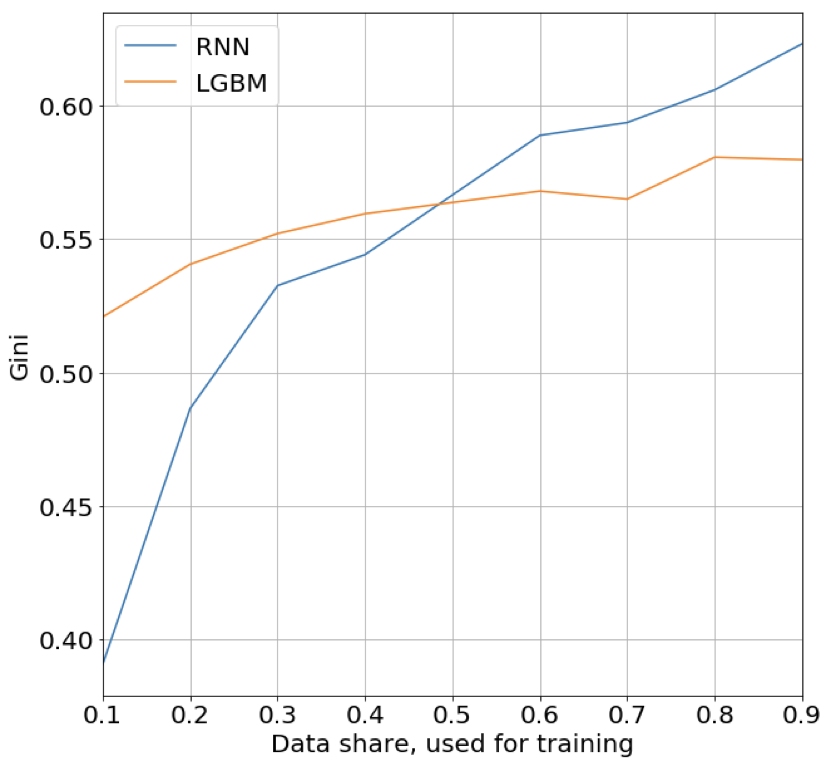
\includegraphics[width=0.46\textwidth]{learning-curve.png}
  \label{fig1}
\end{figure}

On \ref{fig1} there is the learning curve for RNN and LGBM models. As you can see for the small number of training samples LGBM with hand-crafted features is better than RNN but if we have enough data RNN can perform significantly better. Also, RNN has steeper learning curve than LightGBM hence the performance gap would increase with more data.

\section{Model fine-tuning for mortgage loans model}

\section{Results and discussion}

\subsection{Application in production credit pipeline}

\subsection{Interpretation}

While interpretation of the black-box model like LSTM or GRU is exceptionally hard, it is possible to change the architecture of the network to make it interpretable without sacrificing significant part of its classification quality.

One of such changes was proposed by Choi et al.\cite{DBLP:journals/corr/ChoiBSSS16} by the name of RETAIN. The idea is that RNN is not used to perform encoding of the multivariate time-series but instead generates attention weights for each input vector. Then that weights are used to calculate linear combination of input vectors which is finally used for classification.

It is possible to calculate contribution of each input vector to the final prediction. It is possible to apply RETAIN or similar approach to change the architecture of our model.

\subsection{Conclusions}

Neural network based model is hungry for data but can outperform classical ML approaches. The other huge advantage of the neural net based approach is unsupervised feature learning. There is almost no need to manually design features which saves tons of time for the data scientist.

+ Regularization 

The main disadvantage of the neural net based approach is its black-box nature. However, this is the active topic of the research. Some approaches to interpretation like RETAIN can already shed some light to the inner logic of the model.

\bibliographystyle{abbrv}
\bibliography{sigproc}

\end{document}
